\begin{figure}[H]
	\centering
	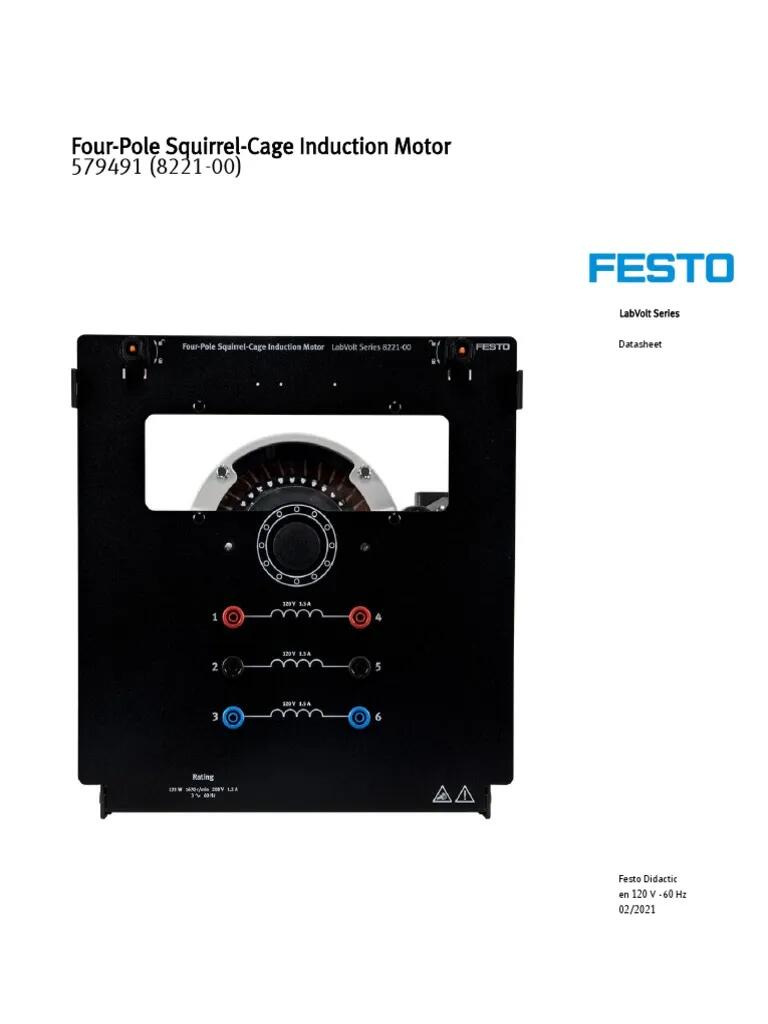
\includegraphics[scale=0.25]{Pictures/Squirrel_Cage}
	\caption{Squirrel Cage Motor}
\end{figure}
\begin{table}[!htp]\centering
	\caption{Squirrel Cage Induction Motor, 8221}\label{tab:motor}
	\setlength{\tabcolsep}{2pt}
	\resizebox{\textwidth}{!}{
		\begin{tabular}{lcccccccccll}
			\toprule
			& & \multicolumn{7}{c}{\textbf{POINT TYPE}} & & & \\ \cmidrule(lr){3-9}
			& & \multicolumn{6}{c}{\textbf{Hardware Point}} & \multicolumn{1}{c}{\textbf{Virtual Point}} & & & \\ \cmidrule(lr){3-8}\cmidrule(lr){9-9}
			\textbf{Point Description} & \textbf{Origin Address} & \textbf{DO} & \textbf{DI} & \textbf{AO} & \textbf{AI} & \textbf{Pwr} & \textbf{Mech Pt} & & \textbf{Destination Address} & \textbf{Destination Description} & \textbf{Notes} \\ \midrule
			\textbf{Squirrel Cage Induction Motor, 8221} & & & & & & & & & & & \\ \midrule
			Phase A Terminal Left & 1 & 0 & 0 & 0 & 0 & 1 & 0 & 0 & 2 & Phase B Terminal Left & Y-configuration \\
			Phase B Terminal Left & 2 & 0 & 0 & 0 & 0 & 1 & 0 & 0 & 1 & Phase A Terminal Left & Y-configuration \\
			Phase B Terminal Left & 2 & 0 & 0 & 0 & 0 & 1 & 0 & 0 & 3 & Phase C Terminal Left & Y-configuration \\
			Phase C Terminal Left & 3 & 0 & 0 & 0 & 0 & 1 & 0 & 0 & 2 & Phase B Terminal Left & Y-configuration \\
			Phase A Terminal Right & 4 & 0 & 0 & 0 & 0 & 1 & 0 & 0 & 14 & Rack, Feeder 2, Red & Y-configuration \\
			Phase B Terminal Right & 5 & 0 & 0 & 0 & 0 & 1 & 0 & 0 & 15 & Rack, Feeder 2, Black & Y-configuration \\
			Phase C Terminal Right & 6 & 0 & 0 & 0 & 0 & 1 & 0 & 0 & 16 & Rack, Feeder 2, Blue & Y-configuration \\
			Squirrel Cage shaft & N/A & 0 & 0 & 0 & 0 & 0 & Belt & 0 &  &  & \\ \bottomrule
		\end{tabular}
	}
\end{table}
